\documentclass[conference]{IEEEtran}
\IEEEoverridecommandlockouts
% The preceding line is only needed to identify funding in the first footnote. If that is unneeded, please comment it out.
\usepackage{cite}
\usepackage{amsmath,amssymb,amsfonts}
\usepackage{algorithmic}
\usepackage{graphicx}
\usepackage{textcomp}
\usepackage{xcolor}
\def\BibTeX{{\rm B\kern-.05em{\sc i\kern-.025em b}\kern-.08em
    T\kern-.1667em\lower.7ex\hbox{E}\kern-.125emX}}
\begin{document}

\title{AiEDA: Agentic AI Design Framework for Digital ASIC System Design}

% \author{\IEEEauthorblockN{Aditya Patra}
% \IEEEauthorblockA{\textit{Department} \\
% \textit{School Name}\\
% Bay Area, California \\
% email address}
% \and
% \IEEEauthorblockN{Saroj Rout}
% \IEEEauthorblockA{\textit{Dept. of Electronics Engineering} \\
% \textit{Silicon University, Odisha}\\
% Bhubaneswar, India \\
% ORCID: 0000-0002-5191-8191 }
% \and
% \IEEEauthorblockN{Arun Ravindran}
% \IEEEauthorblockA{\textit{Dept. of Electrical and Computer Engineering} \\
% \textit{University of North Carolina at Charlotte}\\
% Charlotte, USA \\
% arun.ravindran@charlotte.edu }
% }

\maketitle

\begin{abstract}
\label{sec:abstract}
	The paper addresses advancements in artificial intelligence (AI) and digital chip design, highlighting the integration of Large Language Models (LLMs) in automating hardware description and design. LLMs, known for generating human-like content, are now being explored for creating hardware description languages (HDLs) like Verilog from natural language inputs. This approach aims to enhance productivity and reduce costs in VLSI system design. The study introduces "Aida," a proposed agentic design flow framework for digital ASIC systems, leveraging autonomous AI agents to manage complex design tasks. Aida is designed to streamline the transition from conceptual design to GDSII layout using an open-source toolchain. The framework is demonstrated through the design of an ultra-low-power digital ASIC for KeyWord Spotting (KWS). The use of agentic AI workflows promises to improve design efficiency by automating the integration of multiple design tools, thereby accelerating the development process and addressing the complexities of hardware design.
\end{abstract}

\begin{IEEEkeywords}
 Agentic Flow, Generative AI, Digital design, ASIC, Keyword Spotting (KWS)
\end{IEEEkeywords}
\section{Introduction}
\label{sec:introduction}

The development of Generative AI (GenAI) Large Language Models (LLMs), coupled with the easy API based accessibility of powerful models with hundreds of billions of parameters,  has brought significant advancements in artificial intelligence, allowing systems to generate human-like content across various mediums, including text, images, and code \cite{intro2LLM}. Meanwhile, digital chip design is becoming increasingly complex, requiring management of millions to billions of transistors while optimizing performance, power consumption, and area. Furthermore, it demands precise coordination of design factors such as timing, signal integrity, and manufacturability, all within stringent time-to-market constraints. Recent research has investigated the application of LLMs in digital design, particularly in generating hardware description languages (HDLs) such as Verilog from natural language design descriptions. The use of LLMs in VLSI system design is part of a larger effort by the research community to improve designer productivity, and costs needed to realize complex System-on-Chips (SoCs) \cite{ajayi2019openroad}.

In the last year or so, agentic AI workflows have emerged, where autonomous AI agents perform specific tasks within defined parameters [REF]. Agentic AI systems are defined by their capacity to take actions that consistently work toward achieving goals over time, even when their behavior is not pre-programmed in advance. Agents utilize an LLM to reason and determine the sequence of actions to take. Figure \ref{fig:agentic_overview} shows the high-level outline of an agentic workflow.  These workflows are increasingly used in software design to automate tasks such as code generation, debugging, and testing, thus improving development speed and minimizing human error. While agentic AI workflows have proven effective in software code generation, applying these techniques to hardware design presents additional complexities. This is due to the diverse range of tools required to meet functional and timing correctness, in addition to physical constraints in hardware systems.


\begin{figure}[htbp]
	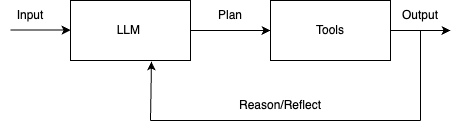
\includegraphics[width=0.45\textwidth]{figs/agentic_overview.png}
	\caption{Agentic AI workflow involves an iterative process involving one or more LLMs for reasoning, and planning, and one or more external tools to execute actions. The input could be a design specification in natural language, or a behavioral description in an HDL. The output could be HDL, netlist, or a GDS layout.
}
	\label{fig:agentic_overview}
\end{figure}

In this paper, we propose Aida, an agentic design flow framework in the design of a digital ASIC system from concept to GDSII using an open source tool flow. Our premise is that the use of agentic AI workflows in digital design would greatly increase designer productivity, enabling rapid implementation of design ideas that integrate a number of different design tools, to generate a full system design is ready to be fabricated. We demonstrate the use of the proposed framework, via the design of a ultra low power digital ASIC for KeyWord Spotting(KWS) architecture. 

The paper is organized as follows. In Section \ref{sec:related_work}, we briefly review the literature on the use of generative AI in hardware design. 
%In Section \ref{sec:background}, we provide a background on agentic AI workflows and the open source digital design tool flow considered in this work. 
In Section \ref{sec:agentic} , we describe Aida, our proposed agentic AI design framework. In Sections \ref{sec:system_design} and Sections \ref{sec:preliminary_evaluation} we present the KWS architecture, and our initial results in using Aida to design it. In Section \ref{sec:discussion}, we discuss the broader applicability of agentic flow in digital system design, the open research questions that need to be addressed, and our current research efforts in this direction. Section \ref{sec:conclusions} concludes the paper.


\section{Related Work (Arun)}
\label{sec:related_work}
We review previous reported work on the use of Generative AI in chip design. DAVE \cite{dave} and Verigen \cite{verigen} are among the first works to exploit the use of LLMs in HDL generation. Their focus is on improving LLM performance by fine-tuning the open source CodeGen-16B model for Verilog code generation. 

The ChipNemo project \cite{chipnemo} from Nvidia does not directly target the use of LLMs in the design of digital systems. Instead, domain-specific LLMs are designed for supporting tasks such as a chatbot that serves as an engineering assistant, EDA script generation, and bug summarization and analysis. Their efforts are thus complementary to our proposed work. Recognizing the need to augment and fine-tune LLMs for hardware design, the MG-Verilog \cite{mg-verilog} project proposes an open source dataset consisting of over 11,000 Verilog code samples and their corresponding natural language descriptions. MG-Verilog dataset is complementary to our effort, and could be used to make the underlying foundational models more accurate through techniques such as Retrieval Augmented Generation (RAG), and fine tuning.  

In the GPT4AIChip project \cite{gpt4aigchip}, a feedback design loop is proposed consisting of prompting the LLM with human-crafted design examples (few-shot learning) and an evolutionary algorithm-based design space exploration algorithm to explore the designs generated by the LLM.  The LLM generated code for a matrix multiplier (GEMM) is synthesized and evaluated on an FPGA using the Xilinx Vivado HLS tools. The AI design flow proposed by GPT4AIChip can be considered as agentic, their design exploration space is limited, and unlike us it does not target the more complex ASIC design flow with time analysis. 

The AutoChip \cite{autochip} project proposes an automated approach that uses large language models (LLMs) to generate HDL. AutoChip combines conversational LLMs such as GPT4 with feedback from Verilog compilers and simulations to iteratively improve Verilog modules. Starting with an initial module generated from a design prompt, it refines the design based on errors and simulation messages. AutoChip's effectiveness is evaluated using design prompts and test benches from HDLBits, a collection of small circuit design exercises. Although AutoChip can be considered as using an agentic design flow, unlike our system design emphasis, they are limited to small circuits and lack an end-to-end design flow. 

\cite{thakur2024verigen}
 

%\section{Background (Arun)}
\label{sec:background}
\begin{itemize}
    \item Generative AI
    \item Agentic AI
    \item ASIC design flow
\end{itemize}
\section{Proposed Agentic AI Design Framework}
\label{sec:agentic}

In this Section, we describe AiEDA, our proposed agentic AI based design framework for digital ASIC system design. Figure \ref{fig:agentic_designflow} shows the proposed design  framework. The design flow is broadly divided into four interrelated stages: 1) Architecture design (shaded orange), 2) RTL design (shaded yellow), 3) Netlist synthesis (shaded red), and 4) Physical design (shaded purple). At each stage, the design is driven by a combination of LLM and appropriate EDA tools operating in a feedback loop. Inputs to the LLMs include design prompts, which instructs the LLM to follow a particular set of actions, or reflection prompts which instructs the LLM to analyze the results of an action. Additionally, the capabilities of LLMs are enhanced with Retrieval Augmented Generation (RAG) techniques, where retrieval of appropriate knowledge (for example, Verilog code dataset such as MG-Verilog) provides a richer context to the LLM in generating a more accurate response. Furthermore, custom LLMs could be employed that have been fine-tuned with domain-specific datasets.


During the architecture design phase, the developer starts with a high-level system specification. They use a large language model (LLM) to decompose the system into individual components and generate a Python model representing these components. This Python script interacts with APIs for custom tools (e.g., MATLAB toolboxes via the MATLAB Engine API) and performance models. The results are then analyzed by another LLM to inform adjustments to the overall system design. This iterative design loop is repeated to evaluate trade-offs between design metrics, such as area and accuracy. The developer can intervene at any point by refining the LLM prompts to guide the design process according to their expertise.

In the RTL design phase, the architectural design in Python, design prompts from the designer, and Verilog code data generated using Retrieval Augmented Generation (RAG) are provided to an LLM, which generates Verilog RTL for the design along with the necessary test benches. Functional verification is performed using the open-source Icarus simulator, and the output is analyzed by the LLM. The LLM identifies failures and generates the necessary modifications to the Verilog code. This feedback loop is repeated until functional verification is successful. As in the architectural design phase, the designer can intervene at any point to modify the prompts, Verilog RTL, or test benches to guide the design toward a desired outcome.

In the Netlist synthesis phase, the Verilog RTL code is synthesized into a gate-level netlist using the open-source Yosys synthesizer, based on standard logic gates from the target process technology library. Timing analysis is then performed using the open-source OpenSTA static timing analyzer. Any timing violations are analyzed by an LLM, and a second LLM generates corrective actions to optimize the timing paths. This is followed by re-running the synthesis with adjusted constraints or updated RTL. 
%As this step can be resource-intensive, the designer may apply an Engineering Change Order (ECO) to resolve minor issues efficiently.

In the Physical design phase, the design's physical layout is created using tools from the open-source OpenROAD tool suite for backend tasks such as placement, clock tree synthesis, routing, and optimization \cite{ajayi2019openroad, ajayi2019toward}. OpenROAD utilizes multiple feedback mechanisms, including Design Rule Check (DRC) feedback, timing analysis feedback, power analysis feedback, and area feedback. Integrating agentic AI into these feedback loops is a potential area for future exploration. The final step uses the open-source Magic tool to generate GDSII files, which are then used for chip fabrication.




\section{System Design (Saroj)}
\label{sec:system_design}
\begin{itemize}
    \item KWS design
    \item Figure
\end{itemize}

%%% FIGURE: KWS ARCHITECTURE
%%% ------------------------
\begin{figure}[htbp]	
    %\centerline{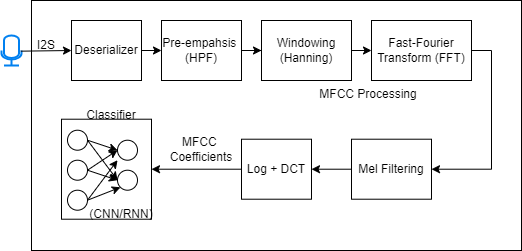
\includegraphics{figs/KWS-architecture.png}}
    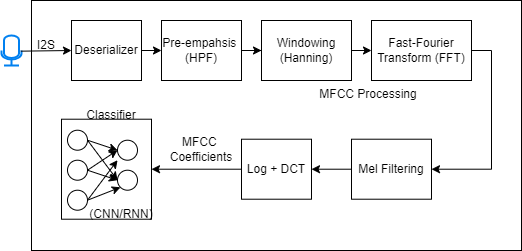
\includegraphics[width=0.45\textwidth]{figs/KWS-architecture.png}
    \caption{Implementation of a Keyword Spotter (KWS)}
    \label{fig:KWS_Arch}
\end{figure}

%%% ------------------------
%%% RTL-to-GDS Design Flow
%%% ------------------------
\subsection{RTL-to-GDS Design Flow}

%%% FIGURE: RTL-TO-GDS Desing Flow 
%%% ------------------------
\begin{figure}[htbp]
	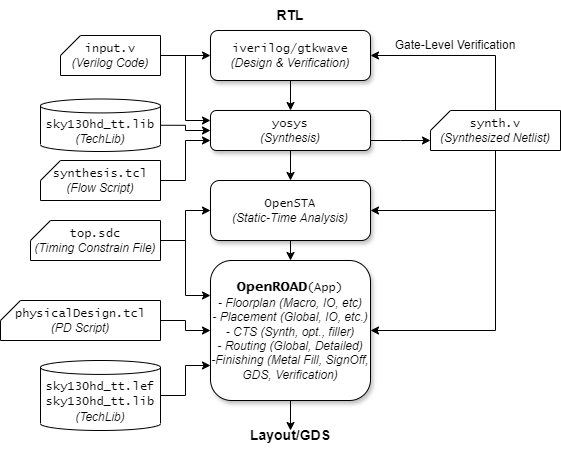
\includegraphics[width=0.45\textwidth]{figs/rtl2gds-toolchain.png}
	\caption{RTL-to-GDS design flow using open-source tool flow.}
	\label{fig:RTL-to-GDS}
\end{figure}


\section{Preliminary Evaluation}
\label{sec:preliminary_evaluation}
In this section, we present a preliminary evaluation of the Keyword Spotting (KWS) architecture using our proposed AiEDA design flow. It is important to note that this work is still ongoing. AiEDA is implemented in Python, with the agentic flow built using the LangGraph framework from LangChain \cite{langgraph}. The design tools referenced are those described in Section \ref{sec:agentic}. The Large Language Model (LLM) utilized in this evaluation is OpenAI's GPT-4o model. As the design tools are still in active development, we plan to release the project as open-source once the code has reached a stable and mature state.

\subsection{AiEDA - Design specification to GDS}

Our initial goal was to validate the AiEDA design flow from RTL to GDS using a relatively simple component. The RTL, synthesis, and netlist stages of AiEDA (refer to Figure Section \ref{sec:agentic}) were tested by designing a 6-bit, 32-depth FIFO. The design process began with a prompt specifying the FIFO's requirements and concluded with the generation of the GDSII layout. The Sky130 standard cell library and PDK from SkyWater Technologies were utilized for this implementation.

\subsection{AiEDA - Architecture design}
We note that despite the popularity of the KWS architecture, hardware implementation can differ greatly depending on the application, which involves various trade-offs between power, area, and accuracy.
For this work, a \textit{smart microphone } application was examined in which the KWS is intended to be embedded directly into the microphone. This configuration allows it to recognize one or more keywords with moderate accuracy, consuming minimal power and occupying a small footprint. Each component is evaluated to determine how its design can be optimized for the specific application.

Digital microphones are generally built to record audio frequencies up to 22~kHz with a sample precision ranging from 12-16 bits. The initial design prompt captured the requirements, and instructed the LLM to explore the bandwidth and precision requirements. The open-source audio tool \textit{Audacity} was incorporated into the design flow using the \textit{ mod-script-pipe} plugin. The reflection prompt directed the LLM to optimize the bandwidth such that the total power of the input signal retains at least 90\% of its original power. Additionally, it instructed the LLM to optimize the bit-width precision ensuring that the tonal component (derived from the FFT operation) within the bandwidth remains largely unaffected."
 After multiple iterations, a 4 kHz bandwidth and 7-bit fixed-point precision were found sufficient for the operation. The Nyquist sampling frequency, which is twice the bandwidth, will decrease from 44 kHz to 8 kHz, leading to an approximately 5x reduction in power consumption. Additionally, using 7-bit precision will yield around a 2x reduction in both area and power consumption.

Next, we designed the individual architectural components shown in Figure \ref{fig:KWS_Arch}. An iteration of the design similar to the overall system was performed for the HPF. The LLM was instructed (Eq.~\ref{eq:hpf}) to select an $\alpha$ that can be implemented using a simple shift-and-add operation, eliminating the need for a hardware multiplier. Following reflection by the LLM, the final design chose an $\alpha = 31/32 = 0.969$ that resulted in an insignificant DC component (first 1-2 bins of the FFT) without a significant loss of audio spectrum. 

A Hanning window was selected for the windowing function, and the LLM was instructed to design approximate coefficients exclusively using single-shift operations such that the limit spectral leakage is limited to 10\%. The output spectrum was analyzed using a Python based script. Following reflection, the LLM precomputed the coefficients in fixed-point form, generating values that can be efficiently approximated by bit-shifts (i.e., powers of 2).

FFT is the largest hardware component with respect to area and power consumption. The $Radix-2^2$ single delay feedback ($R2^2SDF$) is a design that is efficient in both area and power usage, since it uses the fewest multipliers and adders compared to other FFT hardware implementations \cite{chong20220}. The output \textit{spectrogram} was analyzed using a Python based script. The LLM was tasked with evaluating FFT sizes ranging from 16-point to 256-point to identify the minimum number of points that would limit accuracy loss to within 25\%. Upon analysis of the spectrogram, the LLM determined that a 32-point FFT provides fewer frequency bins while achieving substantial hardware savings.

Similar hardware reduction strategies were achieved by employing rectangular Mel filter bins as opposed to triangular ones, with only a slight reduction in accuracy. The last process, the discrete cosine transform (DCT), is a multiply-accumulate (MACC) function \cite{chong20220}. Similar to the Hanning procedure, the coefficient multiplications are transformed into a \textit{shift-and-add} method to reduce the complexity of the hardware without greatly affecting the accuracy.

 The host microcontroller then utilizes these MFCC coefficients with neural network-based classifiers such as CNN or RNN to spot the trained keyword.

\subsection{AiEDA - End-to-end design}
Building on the architectural design of the KWS system, we are now working on developing the full end-to-end system. This process starts with the architectural description in Python and will culminate in the GDSII output. Our goal is to complete this before the conference.
\section{Discussion (Saroj and Arun)}
\label{sec:discussion}
\begin{itemize}
    \item Impact
    \item Lessons learnt
    \item Limitations of approach
    \item Future improvements
    \item Other avenues of exploration
\end{itemize}
\section{Conclusions}
\label{sec:conclusions}
In this paper, we have introduced Aida, an agentic AI design framework for digital ASIC design. Aida leverages advanced Generative AI techniques, including agentic workflows that integrate open-source EDA tools, prompt engineering, few-shot learning, self reflection, and retrieval-augmented generation. We have provided initial evaluation results based on the design of a KeyWord Spotter system. As this work continues to develop, we anticipate presenting more comprehensive evaluation findings by the conference.


%\section*{Acknowledgment}

\bibliographystyle{IEEEtran}
\bibliography{references}


\end{document}
